\documentclass[compress,red]{beamer}
\mode<presentation>
\setbeamertemplate{navigation symbols}{}
\usetheme{Warsaw}

%\hypersetup{pdfpagemode=FullScreen} % makes your presentation go automatically to full screen

% define your own colors:
%\definecolor{Red}{rgb}{1,0,0}
%\definecolor{Blue}{rgb}{0,0,1}
%\definecolor{Green}{rgb}{0,1,0}
%\definecolor{magenta}{rgb}{1,0,.6}
%\definecolor{lightblue}{rgb}{0,.5,1}
%\definecolor{lightpurple}{rgb}{.6,.4,1}
%\definecolor{gold}{rgb}{.6,.5,0}
%\definecolor{orange}{rgb}{1,0.4,0}
%\definecolor{hotpink}{rgb}{1,0,0.5}
%\definecolor{newcolor2}{rgb}{.5,.3,.5}
%\definecolor{newcolor}{rgb}{0,.3,1}
%\definecolor{newcolor3}{rgb}{1,0,.35}
%\definecolor{darkgreen1}{rgb}{0, .35, 0}
%\definecolor{darkgreen}{rgb}{0, .6, 0}
%\definecolor{darkred}{rgb}{.75,0,0}

%\xdefinecolor{olive}{cmyk}{0.64,0,0.95,0.4}
%\xdefinecolor{purpleish}{cmyk}{0.75,0.75,0,0}

\useoutertheme[subsection=false]{smoothbars}

% include packages
\usepackage{subfigure}
\usepackage{multicol}
\usepackage{amsmath}
\usepackage{epsfig} % Erik: didn't work with Miktex
\usepackage{graphicx}
\usepackage[all,knot]{xy}
\xyoption{arc}
\usepackage{url}
\usepackage{multimedia}
\usepackage{hyperref}
\usepackage{helvet}
\usepackage[polish,english]{babel}
\usepackage[utf8]{inputenc}
\usepackage{multirow}
\usepackage{verbatim}
%\usepackage{geometry}
%\geometry{verbose,letterpaper}
%\usepackage{movie15}
%\usepackage{hyperref}


% Or whatever. Note that the encoding and the font should match. If T1
% does not look nice, try deleting the line with the fontenc.

%\logo{}
\titlegraphic{\scalebox{4}{
    
\includegraphics[height=0.5cm]{../pictures/ohr_logo.eps}~
    
\includegraphics[height=0.5cm]{../pictures/cern_logo.eps}}
}


\title[CERN's FMC kit] % (optional, use only with long paper titles)
{CERN's FMC kit}


\author[Matthieu Cattin] % (optional, use only with lots of authors)
{\mbox{Matthieu Cattin}, \mbox{Evangelia Gousiou}, \mbox{Javier Serrano}, \mbox{Erik van der Bij}, \mbox{Tomasz W\l{}ostowski}}
% - Give the names in the same order as the appear in the paper.
% - Use the \inst{?} command only if the authors have different
%   affiliation.

\institute%[Universities of Somewhere and Elsewhere] % (optional, but mostly needed)
{
  %\inst{1}%
%  BE-CO Hardware and Timing section\\
  CERN, Geneva, Switzerland
 %\and
 %\inst{2}%
 %Department of Theoretical Philosophy\\
 %University of Elsewhere
 }
% - Use the \inst command only if there are several affiliations.
% - Keep it simple, no one is interested in your street address.

\date[ICALEPCS 2013] %(optional, should be abbreviation of conference name)
{ICALEPCS 2013, San Francisco, 9 October 2013}
% - Either use conference name or its abbreviation.
% - Not really informative to the audience, more for people (including
%   yourself) who are reading the slides online

%\subject{Theoretical Computer Science}
% This is only inserted into the PDF information catalog. Can be left
% out.


% If you have a file called "university-logo-filename.xxx", where xxx
% is a graphic format that can be processed by latex or pdflatex,
% resp., then you can add a logo as follows:

%\pgfdeclareimage[height=1cm]{ohr-logo}{ohr_logo.jpg}
%\logo{\pgfuseimage{ohr-logo}}


% Delete this, if you do not want the table of contents to pop up at
% the beginning of each subsection:
\AtBeginSection[]
{
  \begin{frame}<beamer>{Outline}
    \tableofcontents[currentsection]
  \end{frame}
}


% If you wish to uncover everything in a step-wise fashion, uncomment
% the following command:

%\beamerdefaultoverlayspecification{<+->}


\begin{document}

\begin{frame}
  \titlepage
\end{frame}

\begin{frame}{Outline}
  \tableofcontents
  % You might wish to add the option [pausesections]
\end{frame}


% Structuring a talk is a difficult task and the following structure
% may not be suitable. Here are some rules that apply for this
% solution:

% - Exactly two or three sections (other than the summary).
% - At *most* three subsections per section.
% - Talk about 30s to 2min per frame. So there should be between about
%   15 and 30 frames, all told.

% - A conference audience is likely to know very little of what you
%   are going to talk about. So *simplify*!
% - In a 20min talk, getting the main ideas across is hard
%   enough. Leave out details, even if it means being less precise than
%   you think necessary.
% - If you omit details that are vital to the proof/implementation,
%   just say so once. Everybody will be happy with that.



%#####################################################################
%############ SECTION ################################################
\section{Why a new kit}

\subsection*{} % dummy subsection to display dots

%------------ FRAME --------------------------------------------------
\begin{frame}{CERN Beams Controls group - BE/CO}

  \begin{block}{Responsible for}
    \begin{itemize}
%    \item Controls infrastructure for all CERN accelerators, transfer lines and experimental areas
%    \item General services such as machine and beam synchronous timing and signal observation
    \item Specification, design, procurement and operation of electronic modules
    \item Linux device drivers, C/C++ libraries, test programs
    \end{itemize}
  \end{block}

  \begin{block}{Hardware kit}
    \begin{itemize}
    \item Analog and digital I/O
    \item Level converters, repeaters
    \item Serial links, timing modules
    \end{itemize}
  \end{block}

  \begin{block}{Currently, September 2013}
    \begin{itemize}
    \item About 120 module types % -- with just a few engineers
    \item Most are custom designed: only 1 in 4 is commercial
    %% \item 1 in 4 is obsolete
    %%   \begin{itemize}
    %%   \item Can maintain existing installations with a limited stock
    %%   \item No re-ordering or production possible
    %%   \item Mostly because of obsolete components
    %%   \end{itemize}
    \end{itemize}
  \end{block}

%  \begin{block}{Supports other groups}
%    \begin{itemize}
%    \item Beam instrumentation, cryogenics, power converters, etc.
%    \end{itemize}
%  \end{block}

%  \begin{block}{Software}
%    \begin{itemize}
%    \item Linux device drivers, C/C++ libraries, test programs
%    \end{itemize}
%  \end{block}

\end{frame}

%------------ FRAME --------------------------------------------------
\begin{frame}{Motivations to design a new kit}

  \begin{block}{Hard to maintain}
    \begin{itemize}
    \item Large variety of modules (about 120)
    \item Obsolete components/modules
    \item Incomplete/nonexistent documentation
    \item Small engineer team %(spec-> design -> prod -> test -> install -> support)
    \item No re-use strategy (pcb, hdl)
    \item \textit{Ad hoc}/non-standard interfaces %(buses, serial protocols, etc...)
    \end{itemize}
  \end{block}

\end{frame}

%------------ FRAME --------------------------------------------------
\begin{frame}{New approach}

  \begin{block}{Principles}
    \begin{itemize}
    \item Openness of designs
    \item Modularity and re-usability
    \item Compliance with existing standards
    \end{itemize}
  \end{block}

  \begin{block}{Carrier-mezzanine concept}
    \begin{itemize}
    \item Generic platform-dependent carriers
    \item Specific platform-independent mezzanines
    \item Reduce number of supported modules
    \end{itemize}
  \end{block}

  % Reduce the number of supported modules
  % -> more generic modules

  % Modularity and re-use on every layer (hw, gw, sw, test)
  % Code and documentation quality
  % Collection of building blocks
  % -> faster developments

\end{frame}

%------------ FRAME --------------------------------------------------
\begin{frame}{Use standards}

  \begin{block}{Based on standards}
    \begin{itemize}
    \item Bus standards: VME, PCI, PCIe, PXIe
    \item FMC mezzanine card (ANSI/VITA 57.1)
    \item Wishbone FPGA internal bus
    \item Linux device drivers
    \end{itemize}
  \end{block}

  \begin{block}{Contribute to standards}
    \begin{itemize}
    \item Wishbone pipelined mode: \textbf{Wishbone spec} Rev.B4 (2010)
    \item FMC bus Linux driver structure: in \textbf{Linux v3.11}
    \item ZIO Linux framework for DAQ and CTL hardware: \\ \textbf{RFC} made \textbf{to Linux} Kernel list
%    \item White Rabbit: will be in \textbf{IEEE 1588} High Accuracy profile
%    \item Wishbone IP core detection scheme, used in FMC bus
    \end{itemize}
  \end{block}

\end{frame}


%#####################################################################
%############ SECTION ################################################
\section{Kit design}

% Alt. title: Design principles ?

% mention hw design? starting with gateware is awkward?
% hw designs licended under CERN OHL
% ohwr repository

%============ SUB-SECTION ============================================
\subsection{Gateware architecture}

%------------ FRAME --------------------------------------------------
\begin{frame}{Wishbone for modularity}

  \begin{block}{Why Wishbone?}
    \begin{itemize}
    \item Open standard
    \item Simple, % doesn't uses a lot of ressources
    \item Collection of cores already available (OpenCores)
    \end{itemize}
  \end{block}

  \begin{block}{Gateware architecture}
    \begin{itemize}
    \item One or more Wishbone buses
    \item A Wishbone interface on all blocks
    \item Crossbar to interconnect/arbitrate masters and slaves
    \item Design of new cores: VME64x, PCIe, DDR3
    \end{itemize}
  \end{block}

\end{frame}

%------------ FRAME --------------------------------------------------
\begin{frame}{Example: FMC-ADC gateware architecture}

  \begin{center}
    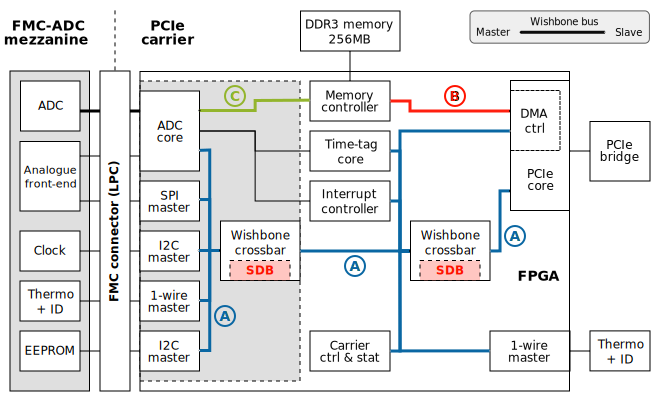
\includegraphics[height=6cm]{../pictures/spec-fmc-adc_arch_simple_color_sdb.eps}
  \end{center}

\end{frame}

%============ SUB-SECTION ============================================
\subsection{Tools and concepts}

%------------ FRAME --------------------------------------------------
\begin{frame}{Gateware design tools}

  \begin{block}{hdlmake}
    \begin{itemize}
    \item Project structure described in \textit{Manifest} files
    \item Solves dependencies
    \item Generates \textit{Makefile} for synthesis and simulation
    \end{itemize}
  \end{block}

  \begin{block}{wbgen2}
    \begin{itemize}
    \item Wishbone slave generator
    \item Structure described in a text file
    \item hdl, C header and documentation automatically generated
    \end{itemize}
  \end{block}

\end{frame}

%------------ FRAME --------------------------------------------------
\begin{frame}{Testing tool}

  \begin{block}{PTS: Production Test Suite}
    \begin{itemize}
    \item Functional test only
    \item Dedicated test setup per board
    \item Software environment to run the tests (Python)
    \item Calibration data stored in FMC EEPROM
    \item Log files (life-cycle management)
    \end{itemize}
  \end{block}

\end{frame}

%------------ FRAME --------------------------------------------------
\begin{frame}{Example: VME boards test system}

  \begin{center}
    \includegraphics[height=6.5cm]{../pictures/pts_rack.eps}
  \end{center}

\end{frame}

%------------ FRAME --------------------------------------------------
\begin{frame}{New concepts}

  \begin{block}{Self Describing Bus}
    \begin{itemize}
    \item Series of predefined structures
    \item Meta-data about cores
    \item Allows software to know about gateware architecture
    \end{itemize}
  \end{block}

  \begin{block}{SDB File System}
    \begin{itemize}
    \item Based on SDB data structures
    \item Easy to parse (e.g. for embedded processor)
    \item Library and tools available % (generate, read)
    \item Used in the FMC EEPROM
    \end{itemize}
  \end{block}

\end{frame}

%------------ FRAME --------------------------------------------------
\begin{frame}[fragile]{Example: SDB record (VHDL)}

  %\begin{block}{SDB record example}
  \small
    \begin{verbatim}
      constant c_ONEWIRE_SDB_DEVICE : t_sdb_device := (
         abi_class     => x"0000",
         abi_ver_major => x"01",
         abi_ver_minor => x"01",
         wbd_endian    => c_sdb_endian_big,
         wbd_width     => x"4",
         sdb_component => (
         addr_first  => x"0000000000000000",
         addr_last   => x"0000000000000007",
         product     => (
            vendor_id => x"000000000000CE42",
            device_id => x"00000602",
            version   => x"00000001",
            date      => x"20121116",
            name      => "WB-Onewire.Control ")));
    \end{verbatim}
    \normalsize
  %\end{block}

\end{frame}

%------------ FRAME --------------------------------------------------
\begin{frame}{FMC EEPROM structure}

  \begin{center}
    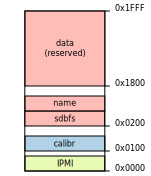
\includegraphics[height=6.5cm]{../pictures/eeprom_struct.eps}
  \end{center}

\end{frame}


% explain fpga fw load (golden -> read eeprom -> final bitstream)

%============ SUB-SECTION ============================================
\subsection{Open Hardware products}

%------------ FRAME --------------------------------------------------
\begin{frame}{Open Hardware products}

  \begin{block}{What is an OH product?}
    \begin{itemize}
    \item Hardware board
    \item FPGA gateware
    \item Linux driver
    \item Production test system
    \end{itemize}
  \end{block}

  \begin{block}{Carriers}
    \begin{itemize}
    \item Three fully supported (SPEC, SVEC, SPEXI)
    \item Six other carriers (VXS, AMC, stand-alone)
    \end{itemize}
  \end{block}

  % VFC, PFC, AFC, RHINO, VXS DSP carrier, Stand-alone 18-slot FMC carrier

  \begin{block}{Mezzanines}
    \begin{itemize}
    \item Four fully supported (ADC-100M, TDC, DIO-5ch, FD)
    \item About a dozen other mezzanines (ADC, DAC, DDS, DIO)
    \end{itemize}
  \end{block}

  % ADC-130M, ADC-200k, ADC-250M, ADC-1G
  % ADC-125M-DAC-600M, ADC-10M-DAC-50M
  % DAC-10M, DAC-130M, DAC-250M, DAC-600M-DDS
  % DIO-16ch, DIO-32ch
  % + others more specific mezzanines

\end{frame}

%------------ FRAME --------------------------------------------------
\begin{frame}{SPEC - Simple PCI Express FMC carrier}{Made in Spain, The Netherlands \& Poland}

  \begin{center}
%    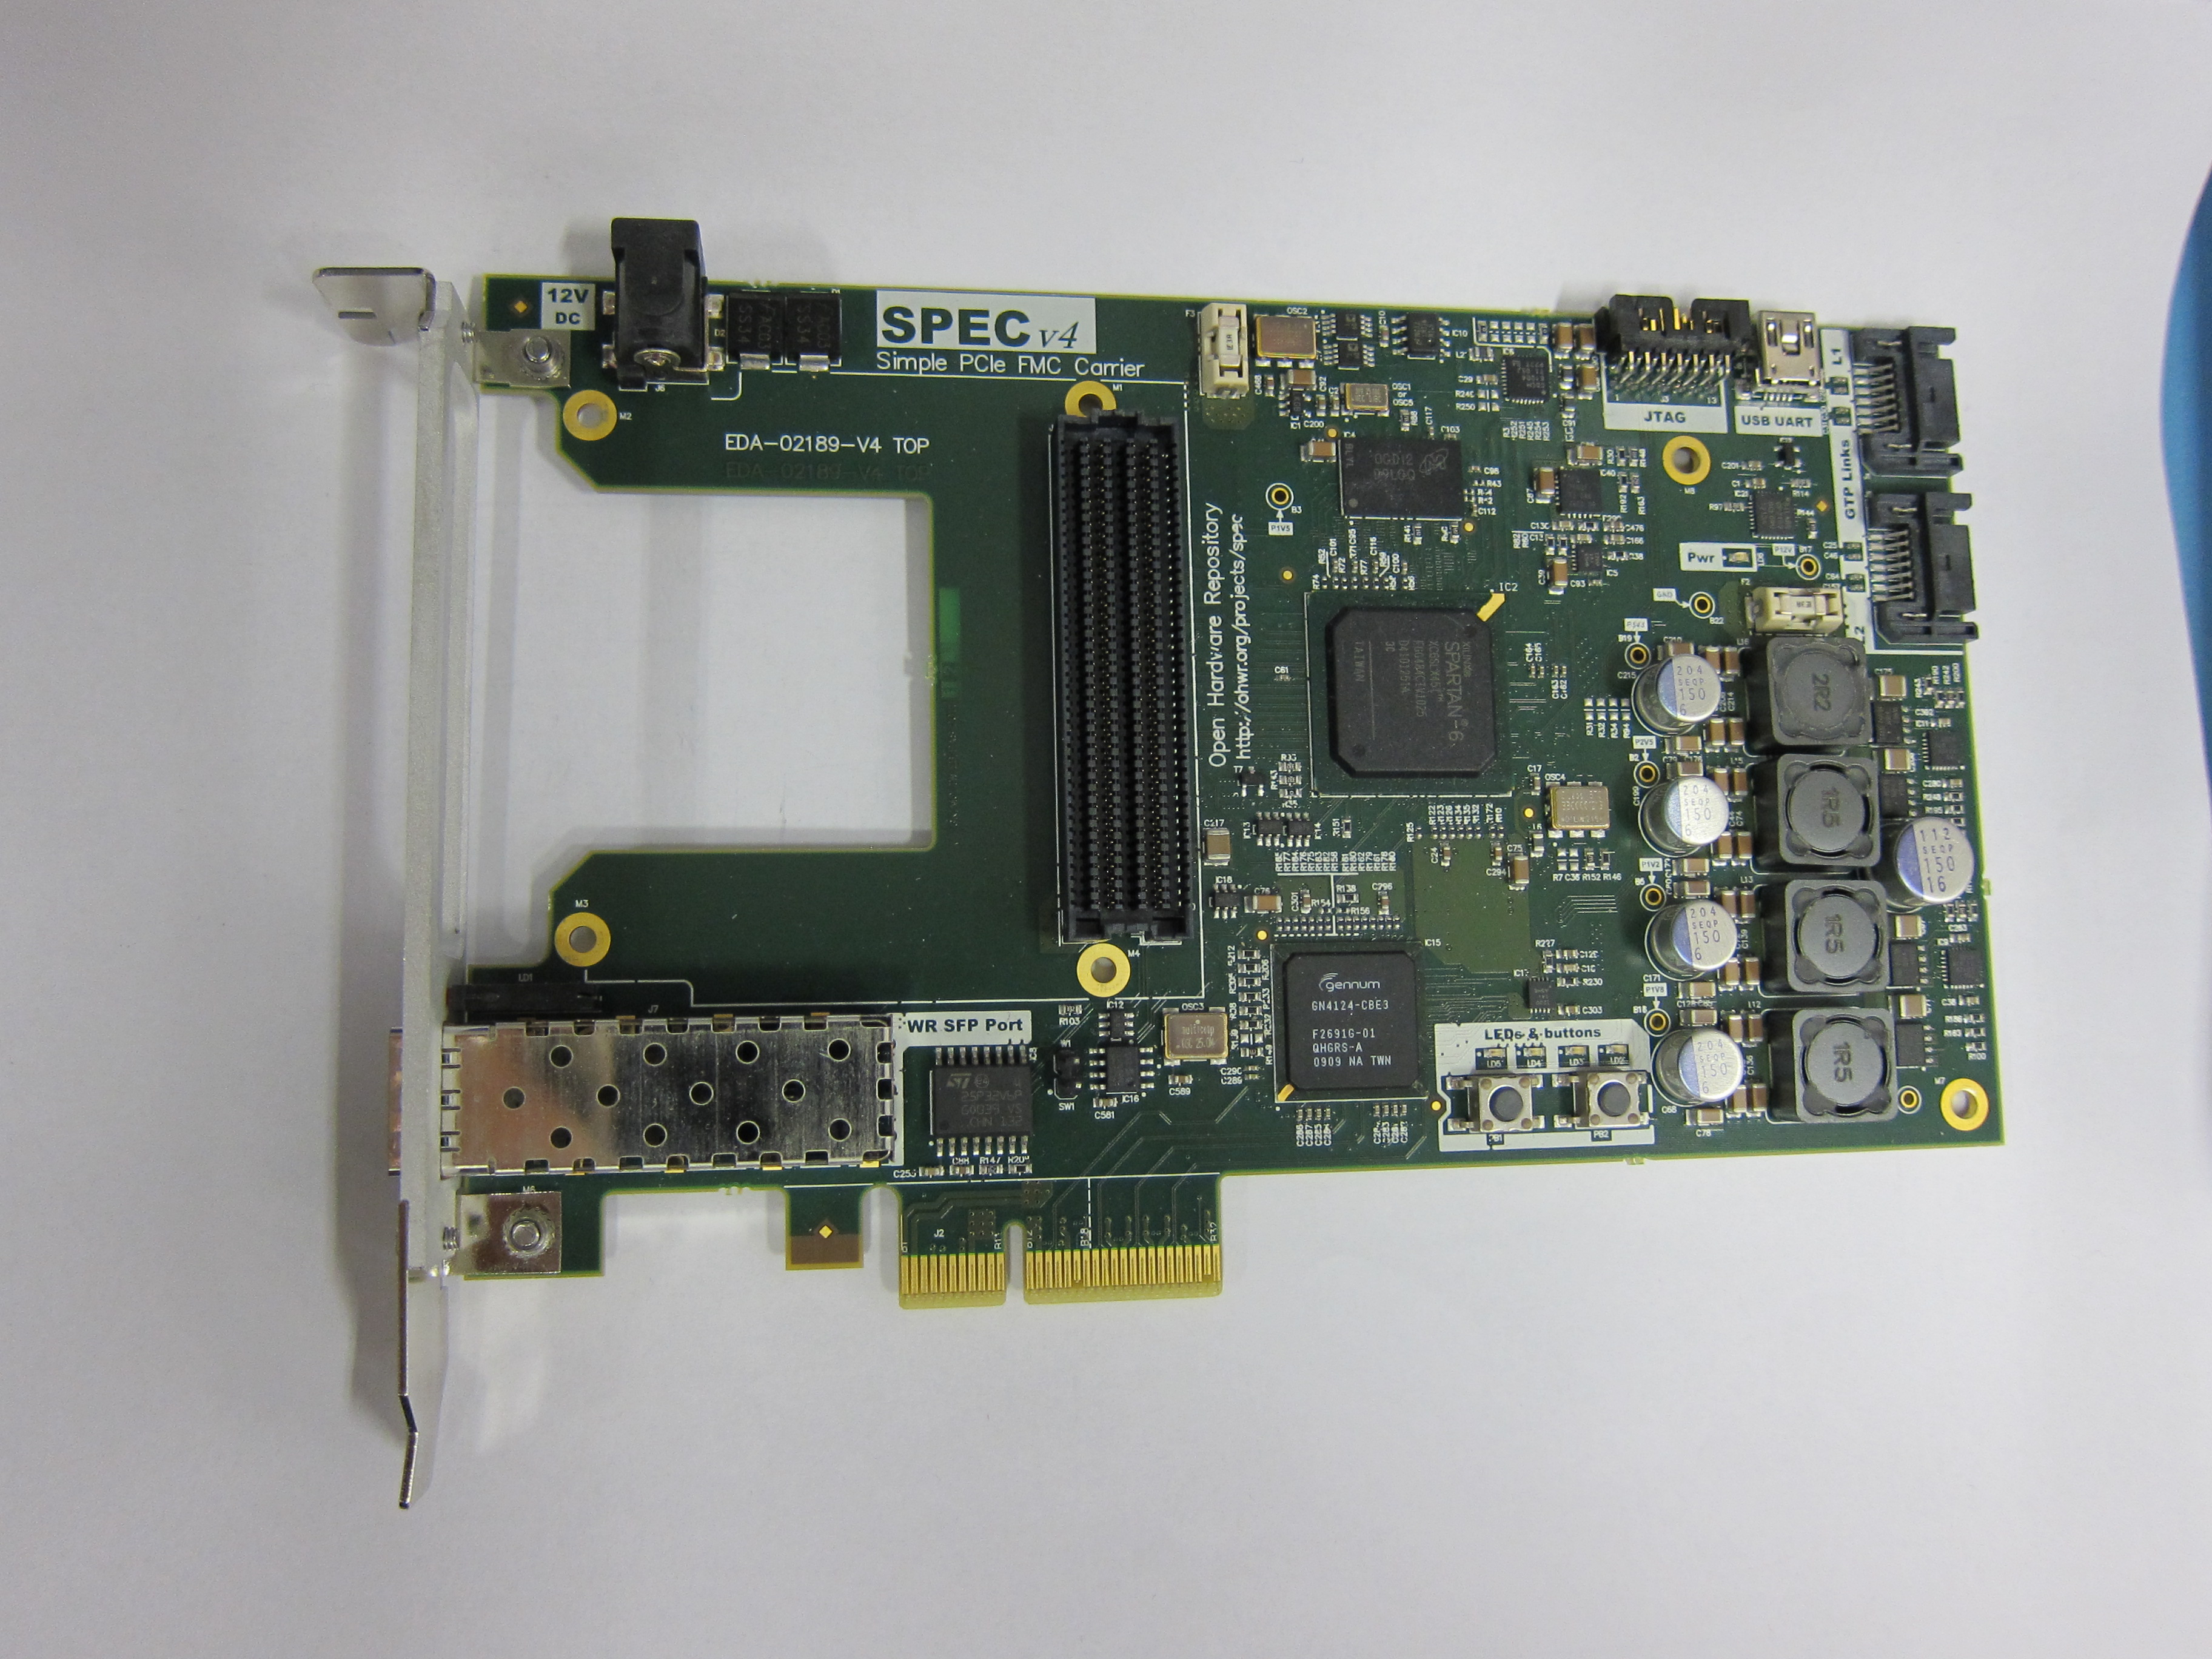
\includegraphics[height=7cm]{../pictures/spec_v4.eps}
  \end{center}

\end{frame}

%------------ FRAME --------------------------------------------------
\begin{frame}{SVEC - Simple VME FMC Carrier}{Made in Germany}

  \begin{center}
%    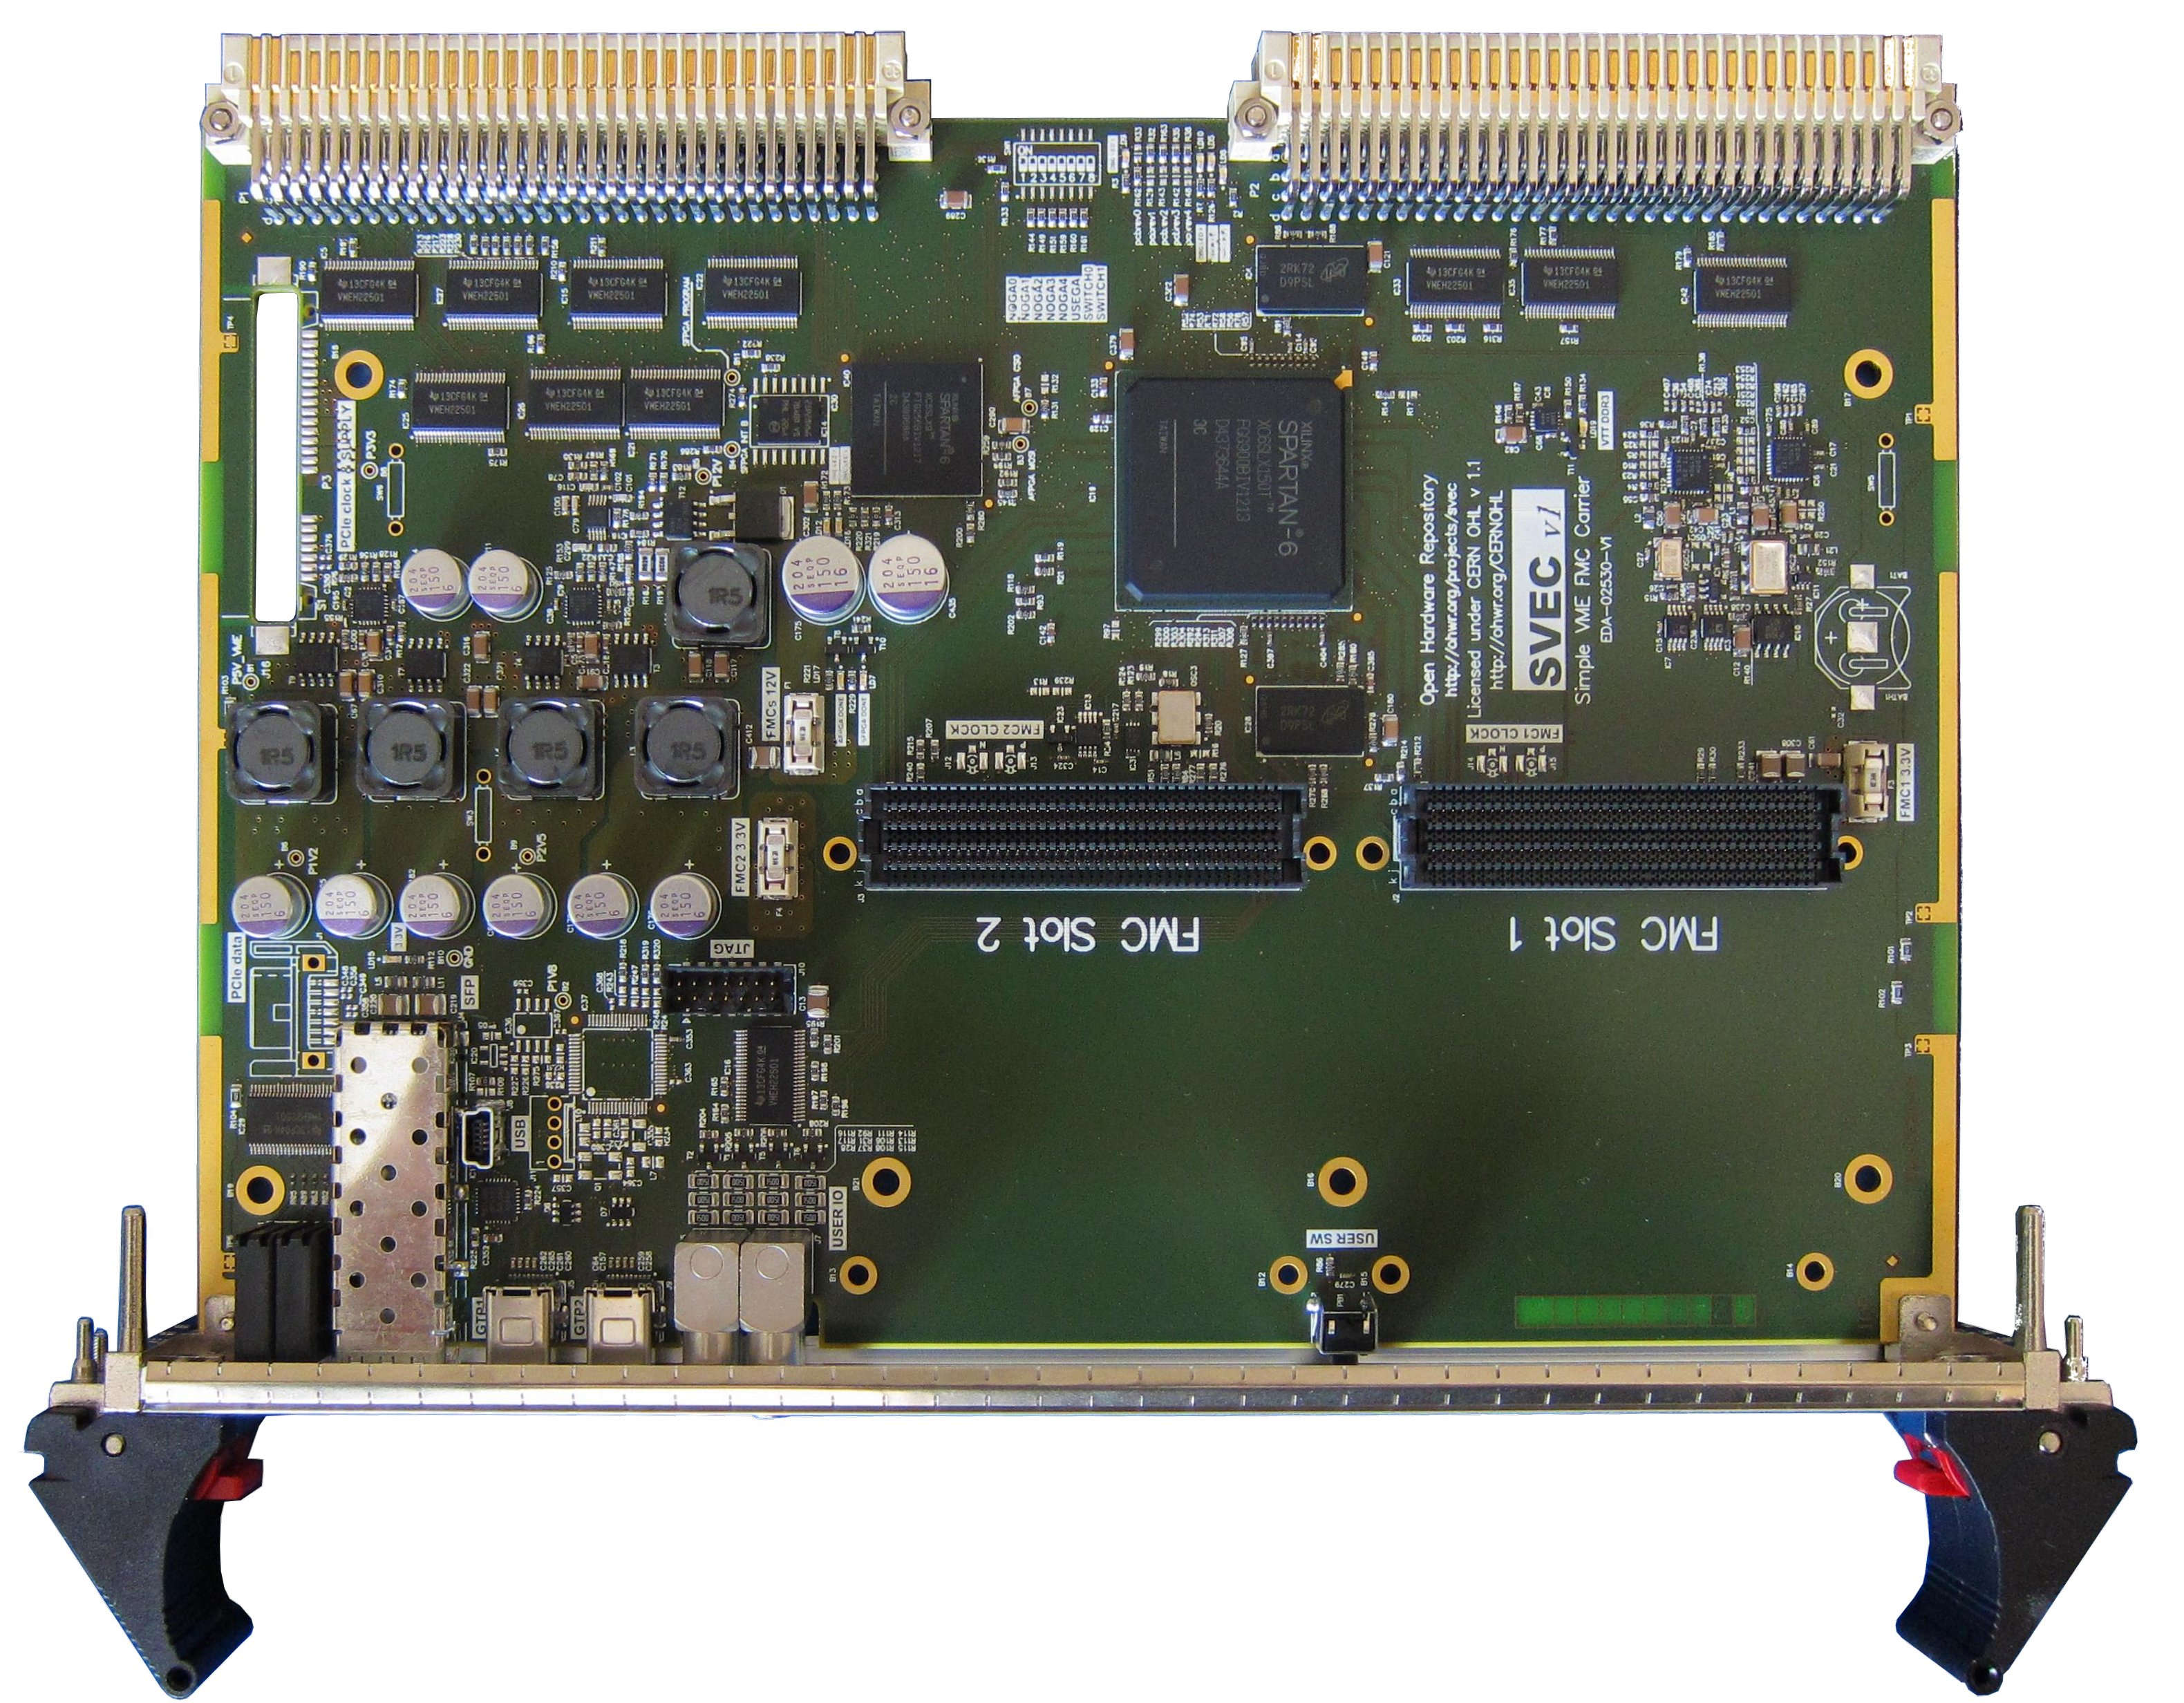
\includegraphics[height=7cm]{../pictures/svec.eps}
  \end{center}

\end{frame}

%------------ FRAME --------------------------------------------------
\begin{frame}{SPEXI - Simple PXI Express FMC carrier}{A modified SPEC board}

  \begin{center}
%    \includegraphics[height=7cm]{../pictures/spexi_v0.eps}
  \end{center}

\end{frame}

%------------ FRAME --------------------------------------------------
\begin{frame}{FMC mezzanine: 5-channel 1ns TDC}{A joint development by TE/ABT, TE/CRG \& BE/CO}

  \begin{center}
%    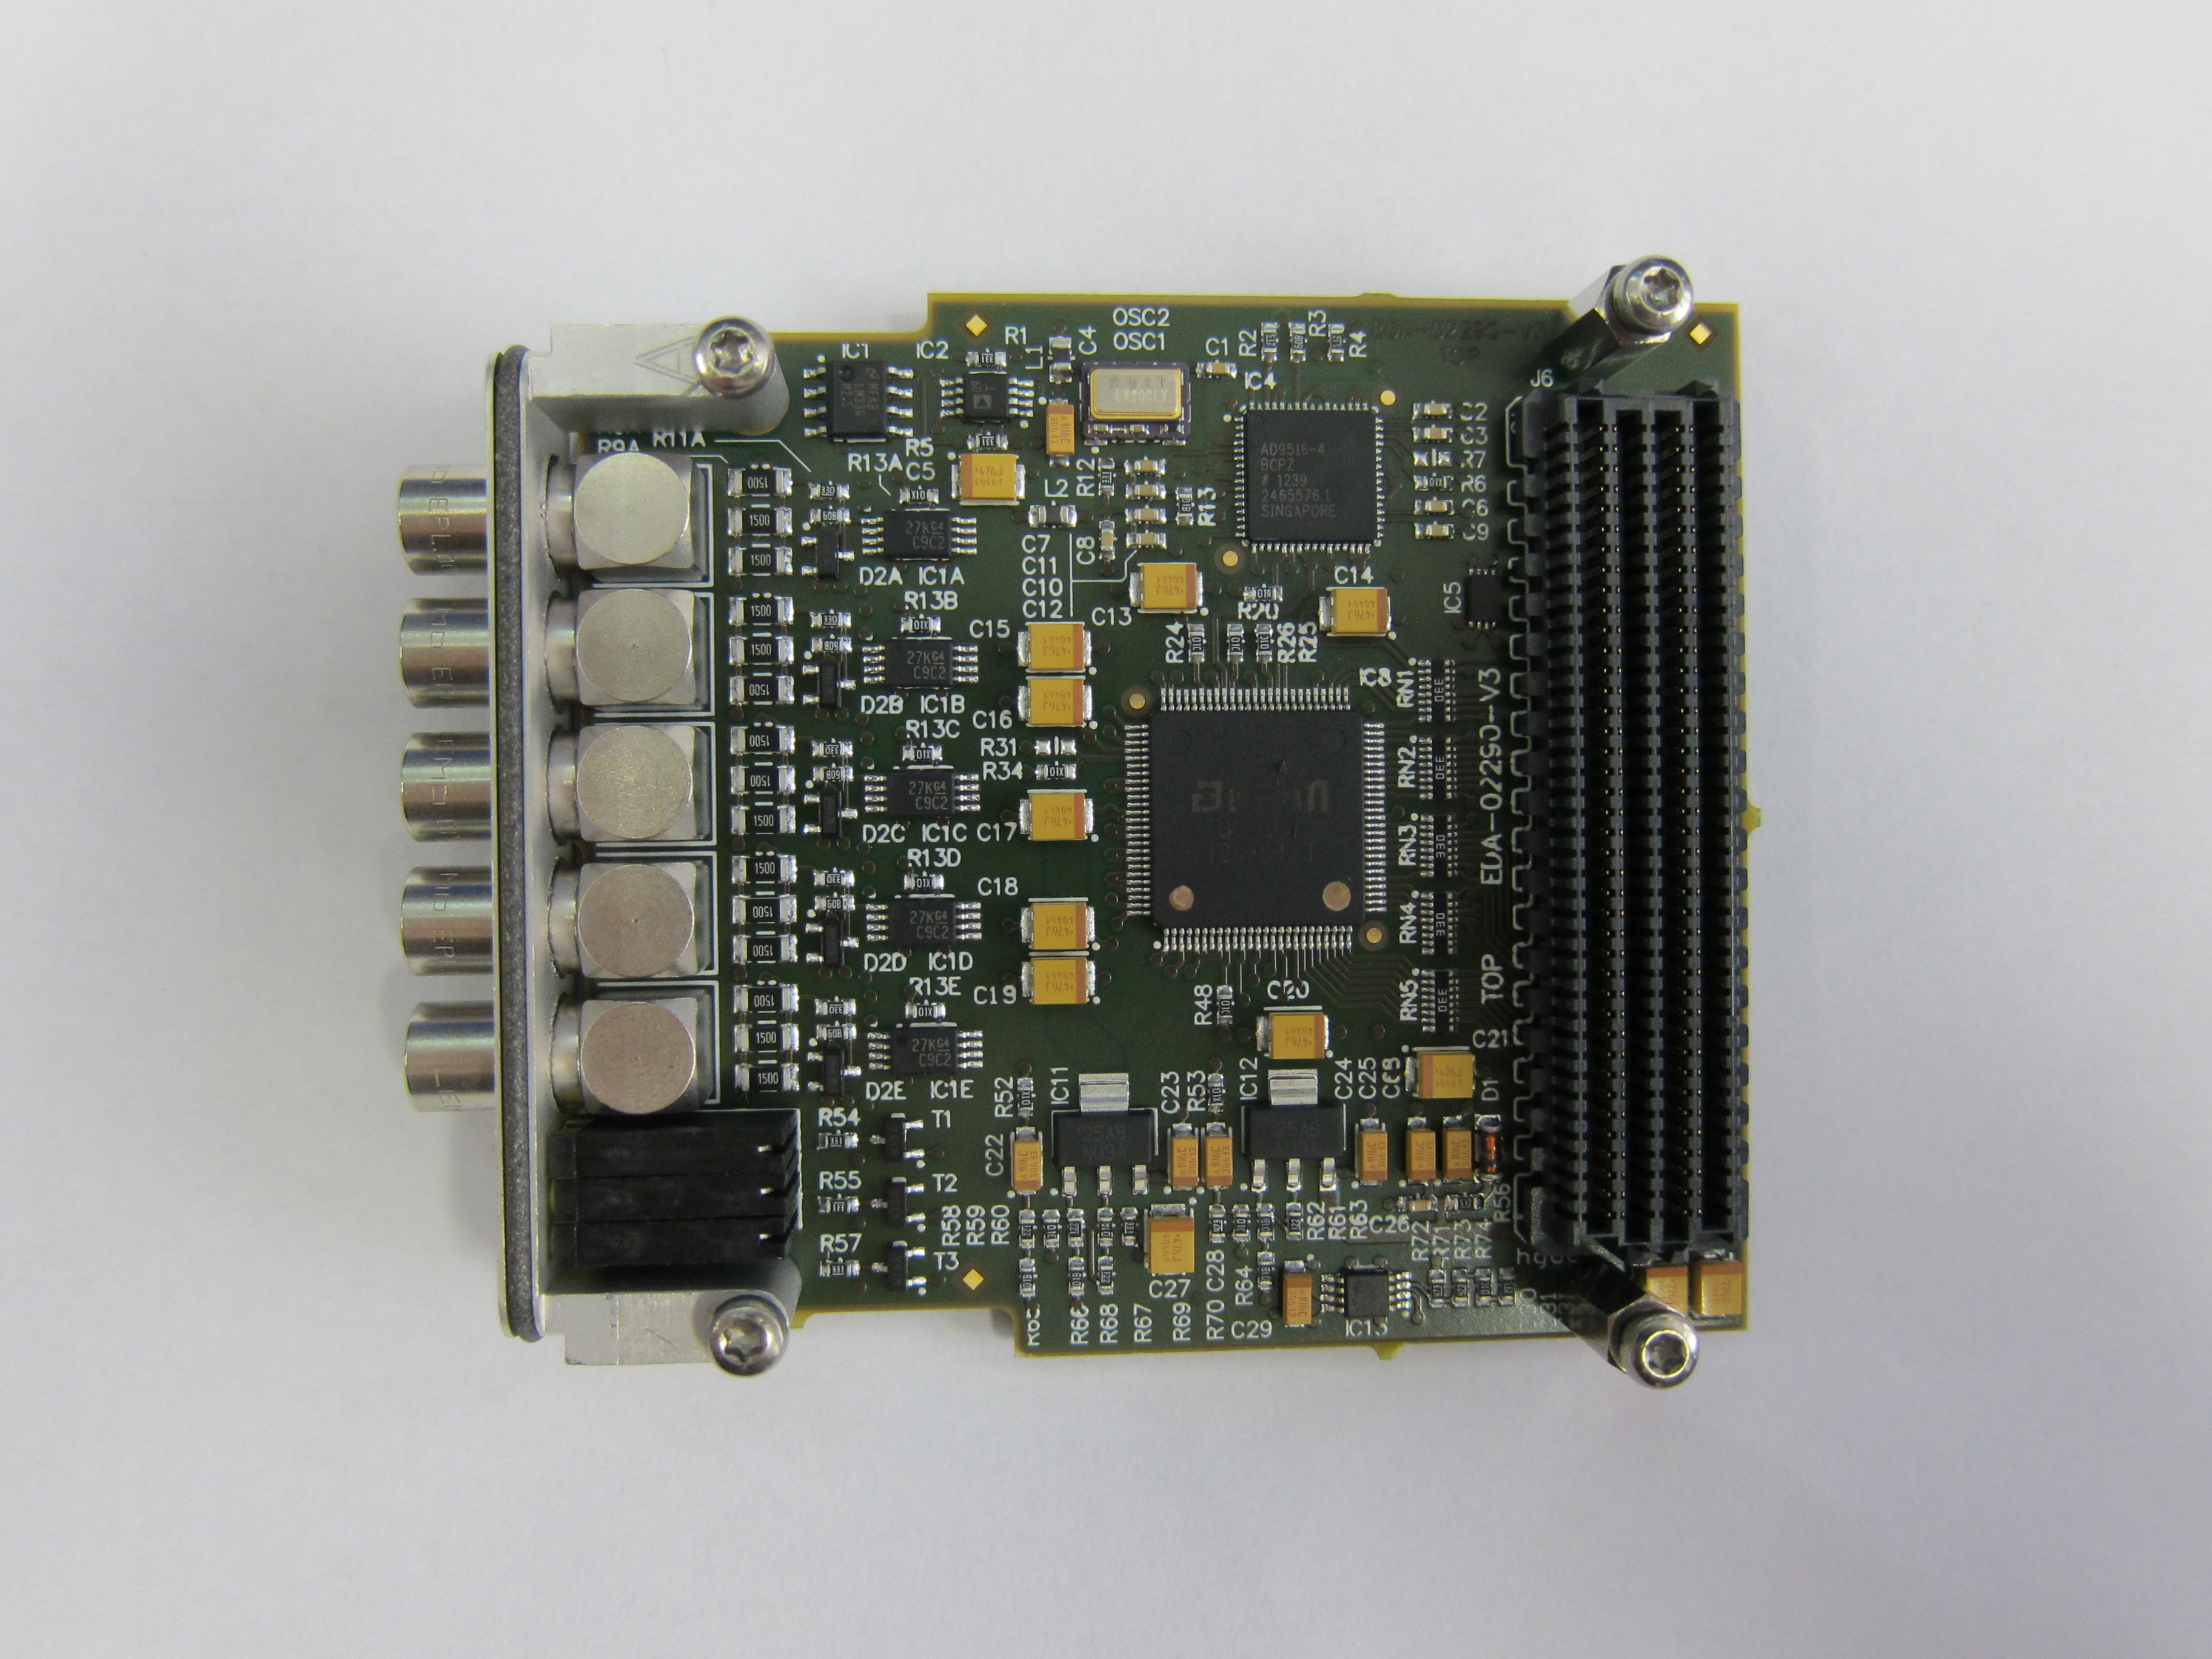
\includegraphics[height=6.5cm]{../pictures/fmc-tdc.eps}
  \end{center}

\end{frame}

%------------ FRAME --------------------------------------------------
\begin{frame}{FMC mezzanine: 100 MSPS 14-bit 4-channel ADC}

  \begin{center}
%    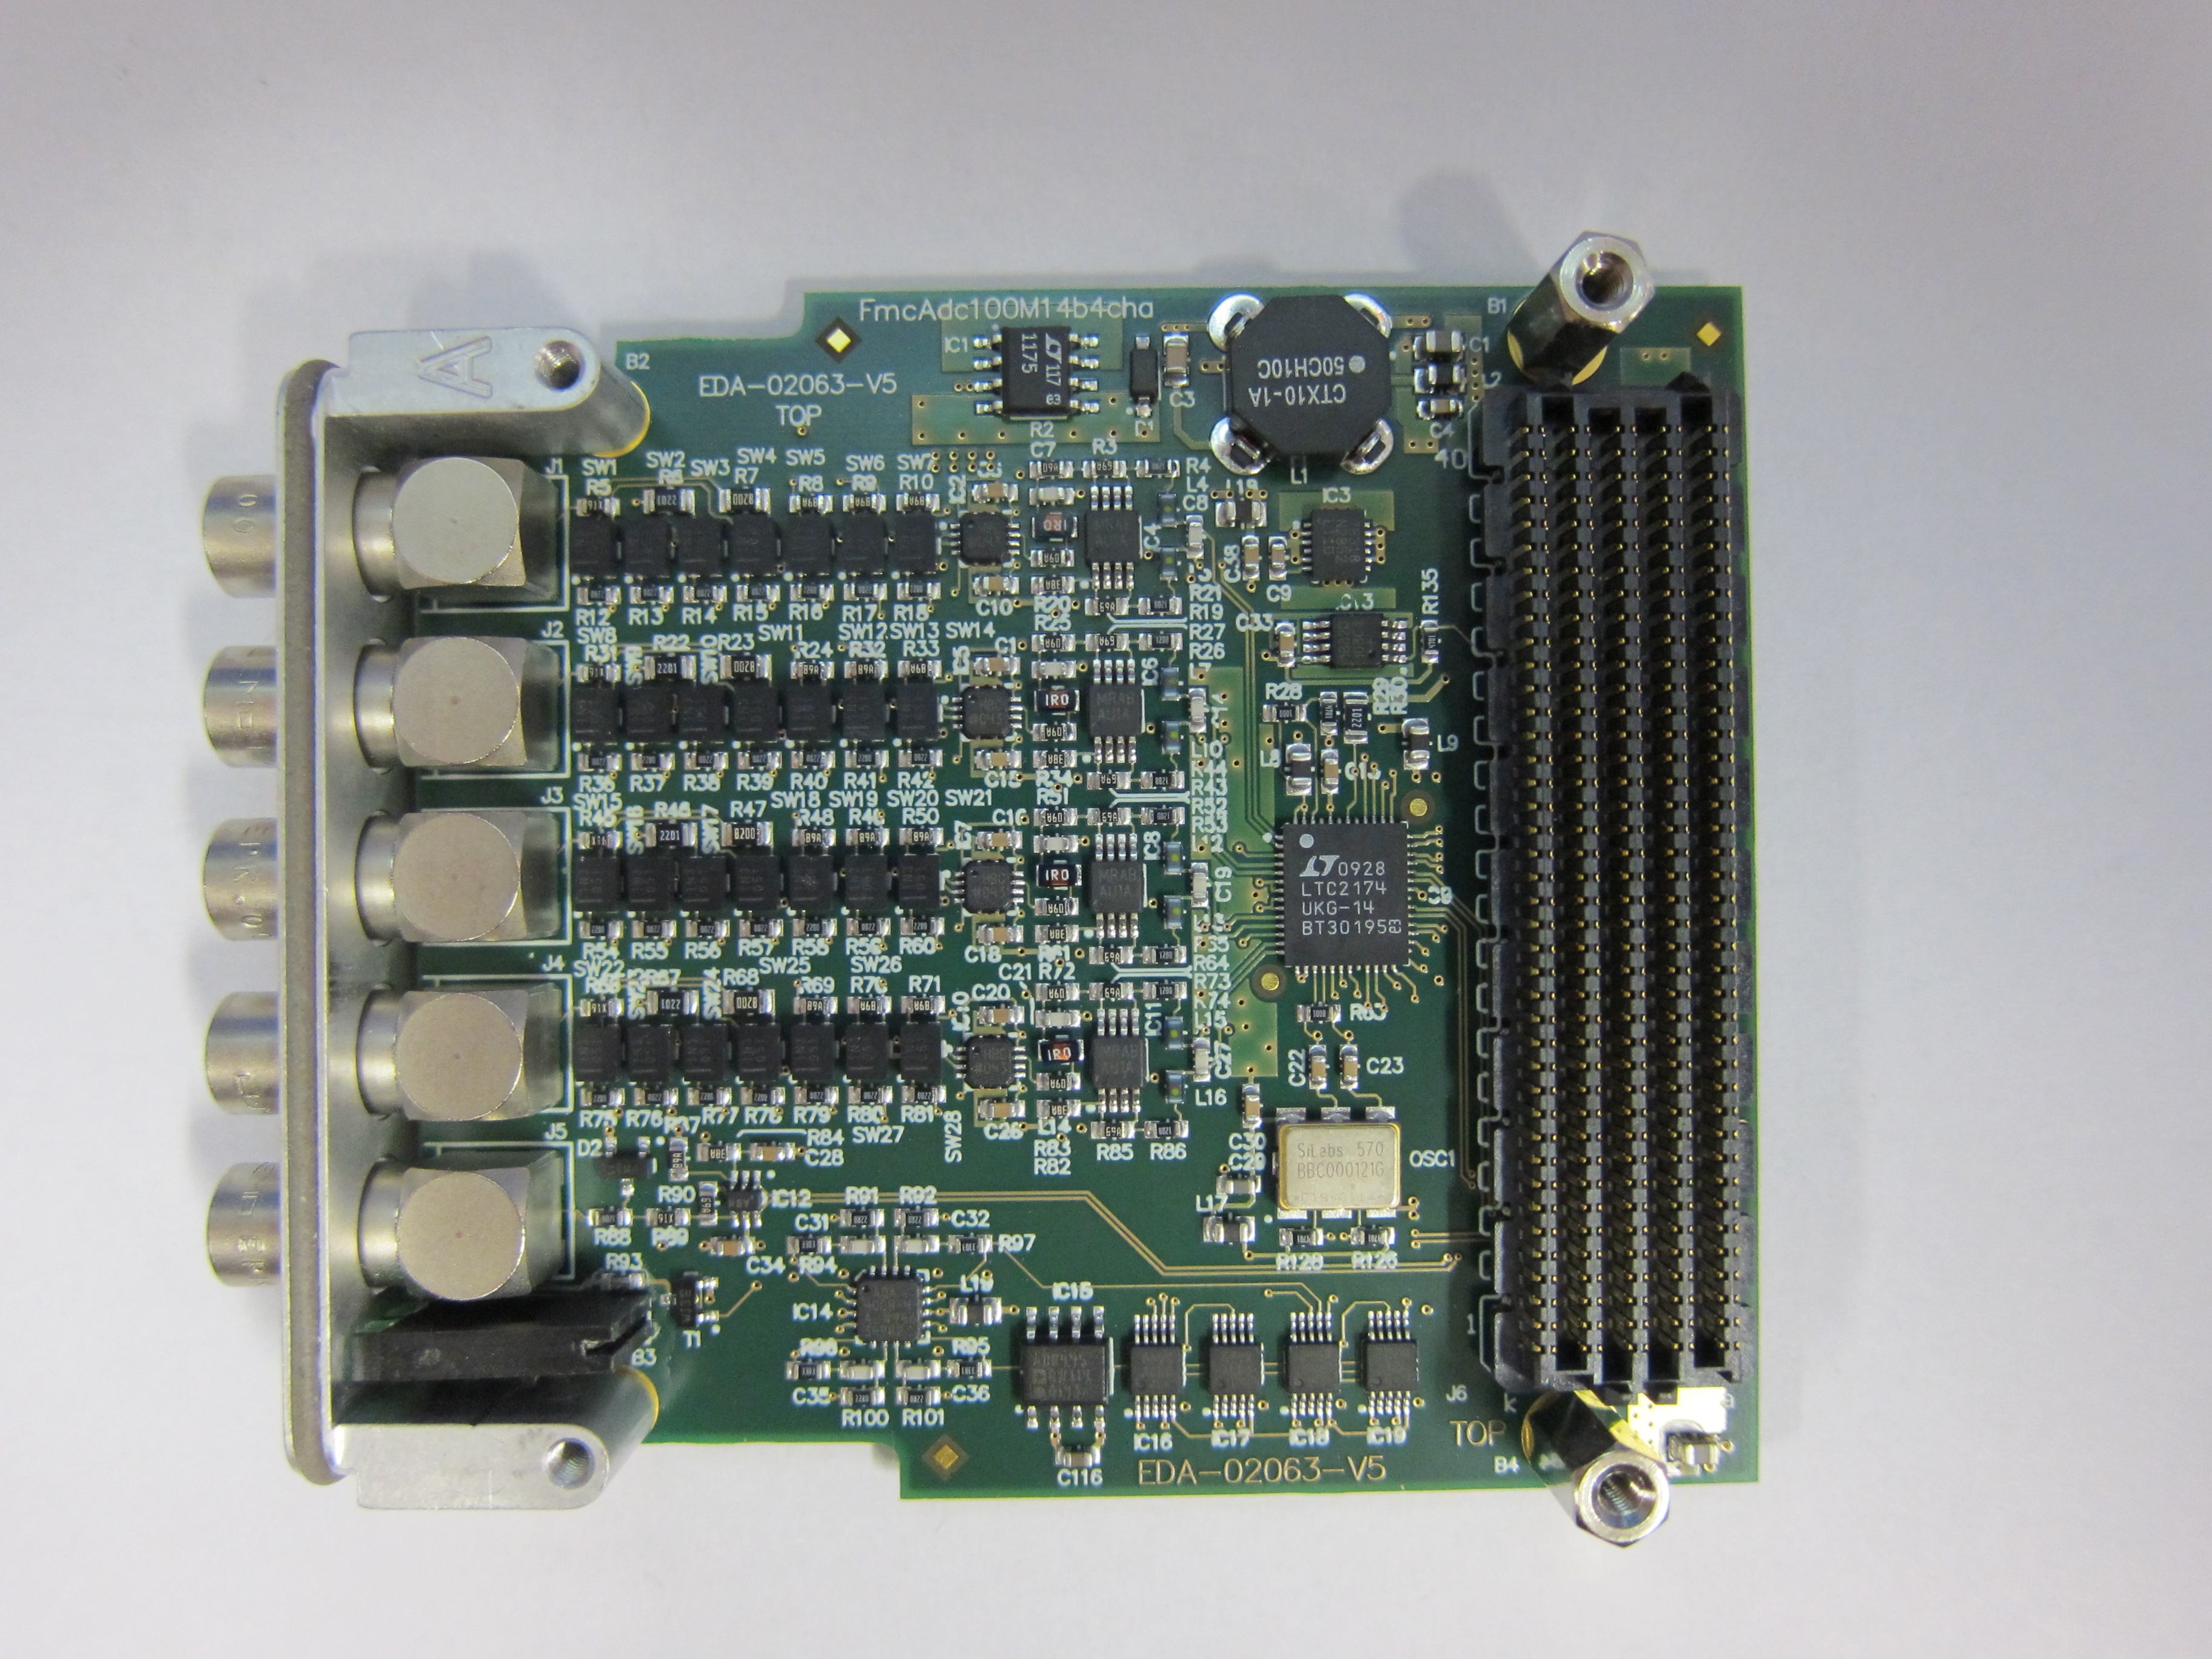
\includegraphics[height=6.5cm]{../pictures/fmc-adc-100m.eps}
  \end{center}

\end{frame}

%------------ FRAME --------------------------------------------------
\begin{frame}{Commercially available CERN OH designs}{September 2013}

  \begin{table}
    \centering

% \begin{tabular}{|l||r|r|r|c|}
    \begin{tabular}{|l||r|r|r|}
      \hline
      Project & Producers & Users & Produced\\
      \hline\hline
      SPEC carrier - PCIe & 3 & 41 & 300 \\
      \hline
      SVEC carrier - VME & 2 & 4 & 105 \\
      \hline
      SPEXI carrier - PXIe & 1 & 2 & (proto) 3 \\
      \hline
      \hline
      ADC 100M 14b 4ch & 2 & 11 & 70 \\
      \hline
      TDC 1ns 5cha & 1 & 3 & 70 \\
      \hline
      FMC DEL 1ns 4cha & 3 & 4 & 108 \\
      \hline
      FMC DIO 5ch & 3 & 10 & 92 \\
      \hline
      \hline
      \textit{WR switch 18 ports} & 1 & 11 & 77\\
      \hline
    \end{tabular}

    \caption{eight CERN OH designs found producers and users}
  \end{table}

\end{frame}

%------------ FRAME --------------------------------------------------
\begin{frame}{Modularity advantages}

  % Or just say it?
  \begin{block}{Easy porting}
    \begin{itemize}
    \item ADC-100M on SPEC = few months
    \item 2x ADC-100M on SVEC = one week
    \end{itemize}
  \end{block}

  \begin{block}{Re-use}
    \begin{itemize}
    \item 
    \item 
    \end{itemize}
  \end{block}

  \begin{block}{}
    \begin{itemize}
    \item 
    \item 
    \end{itemize}
  \end{block}

\end{frame}


%#####################################################################
%############ SECTION ################################################
\section{Open Hardware}

%============ SUB-SECTION ============================================
\subsection{Benefits}

%------------ FRAME --------------------------------------------------
\begin{frame}{Re-use of work}

  \begin{block}{Examples of re-use of work}
    \begin{itemize}
    \item Two companies modified SPEC carrier design
      \begin{itemize}
      \item larger FPGA (for software radio)
      \item AMC and PXIe bus versions
      \end{itemize}
    \item A company modified ADC100M design
      \begin{itemize}
      \item other input filter
      \item high-voltage front-end
      \end{itemize}
%    \item Company re-uses White Rabbit spec for own product.
%    \item Companies re-used White Rabbit core.
%    \item A company re-used nanoFIP code for renovating trains
    \end{itemize}
  \end{block}

\end{frame}

%------------ FRAME --------------------------------------------------
\begin{frame}{Re-use of boards}

  \begin{block}{Our designs are re-used by:}
    \begin{itemize}
    \item Other groups at CERN
    \item Other laboratories/institutes
    \item Universities
    \item ...
    \end{itemize}
  \end{block}

\end{frame}

% merge re-use of work and re-use of boards in one slide?

%------------ FRAME --------------------------------------------------
\begin{frame}{Better designs}

  \begin{block}{}
    \begin{itemize}
    \item Peer review
    \item User feedback
    \item User give bug fixes, not only bug reports
    \item Early bug detection (production by design companies)
    \item Good documentation
    \end{itemize}
  \end{block}

\end{frame}

%============ SUB-SECTION ============================================
\subsection{Collaborations}

%------------ FRAME --------------------------------------------------
\begin{frame}{Collaboration}

  \begin{block}{Board design}
    \begin{itemize}
    \item Specified by CERN
    \item Schematics and layout by company
    \item Reviewed by CERN
    \end{itemize}
  \end{block}

  \begin{block}{Board production and test}
    \begin{itemize}
    \item Offloads CERN team
    \item Warranty, repair of faulty devices
    \end{itemize}
  \end{block}

  \begin{block}{HDL design}
    \begin{itemize}
    \item Core library
    \end{itemize}
  \end{block}

  % WB crossbar dev. in GSI

\end{frame}

%============ SUB-SECTION ============================================
\subsection{Drawbacks} % remove this subsection

%------------ FRAME --------------------------------------------------
\begin{frame}{}

  \begin{block}{}
    \begin{itemize}
    \item Support to collaborators and users, forces to have better documentation
    \item Companies selling OH products, take over support to users
    \end{itemize}
  \end{block}

\end{frame}


%############ SECTION ################################################
\section{Perspectives}

\subsection*{} % dummy subsection to display dots

%------------ FRAME --------------------------------------------------
\begin{frame}{Improving quality}

  \begin{block}{}
    \begin{itemize}
    \item Finish documentation
    \item Clean and unify repositories
    \item Meanwhile, FAQ page
    \end{itemize}
  \end{block}

\end{frame}

%------------ FRAME --------------------------------------------------
\begin{frame}{PCB design tool}

  \begin{block}{Limitation to re-usability}
    \begin{itemize}
    \item No common file format
    \item No adequate FOSS alternative
    \end{itemize}
  \end{block}

  \begin{block}{Improving KiCad}
    \begin{itemize}
    \item CERN giving a push
    \item Efficient PCB design tool
    \end{itemize}
  \end{block}

  % Javier's slide from OKcon
  % Icarus?

\end{frame}

%------------ FRAME --------------------------------------------------
\begin{frame}{New front-end computer platform}

  \begin{block}{Current platforms}
    \begin{itemize}
    \item VME64x
    \item PICMG 1.3 (PCI and PCIe)
    \item PXI Express (supported by EN/ICE)
    \end{itemize}
  \end{block}

  \begin{block}{Limitations}
    \begin{itemize}
    \item Difficult maintainance (PCI, PCIe)
    \item Low bus throughput (VME)
    \item No clock and trigger line on backplanes (VME, PCI)
    \end{itemize}
  \end{block}

%split in two slides!!!

  \begin{block}{Future platform not yet know, but}
    \begin{itemize}
    \item New carrier design
    \item Re-useable mezzanines
    \item HDL and software framework
    \end{itemize}
  \end{block}

\end{frame}


%############ SECTION ################################################
\section{Conclusions}

\subsection*{} % dummy subsection to display dots

%------------ FRAME --------------------------------------------------
\begin{frame}{}

  \begin{block}{The FMC kit is not only a set of hardware module}
    \begin{itemize}
    \item Collection of hdl cores
    \item Linux device driver and test program
    \item Production test system
    \item Tools %(wbgen, hdlmake, )
    \item Commercially available (sometimes from several sources)
    \end{itemize}
  \end{block}

\end{frame}

%------------ FRAME --------------------------------------------------
% Erik's slide with products webpages?



%\vspace{0.2cm}
%Opening up your designs does make you more vulnerable to this disease.
%\end{frame}
%%One slide to justify our license choice so far
%% One slide on evil patents and the risk for open design.

\end{document}


